\section{Wasserfallmodell}

Das \textbf{Wasserfallmodell} löst für \textit{bestimmte} Projekte\footnote{
zu den Grenzen des Wasserfallmodells s. a. Abschnitt~\ref{sec:grenzen-des-wasserfallmodells}
} die Probleme des opportunistischen Vorgehens und ist in \textbf{6 Phasen} aufgeteilt (s. Abbildung~\ref{fig:wasserfallmodell}).\\
Die Ergebnisse der Phasen sind \textit{Dokumente}, \textit{Modelle},\ textit{Code} oder \textit{Testprotokolle}, die man zusammenfassend als \textbf{Artefakte} bezeichnet.\\

\subsection*{Eigenschaften des Wasserfallmodells}
\begin{itemize}
    \item Die Phasen des Wasserfallmodells folgen \textbf{strikt hintereinander}.
    \item Ergebnisse abgeschlossener Phasen werden nicht mehr geändert.
    \item Stellt sich heraus, dass in einer vorhergehenden Phase schwerwiegende Fehler begangen wurden, muss das gesamte Team in diese Phase zurückspringen, den Fehler beheben und von da an jede nachfolgende Phase erneut durchlaufen.
    \item[] $\rightarrow$ Voraussetzung für ein erfolgreiches Arbeiten mit diesem Modell ist eine vollständige und fehlerfreie Erstellung von Artefakten in jeder Phase
    \item \textbf{Vorteile}:
        \begin{itemize}
            \item Bei überschaubaren Projekten bietet das Modell eine genauere Planbarkeit, da spätestens nach dem Entwurf klar ist, welche Arbeiten erledigt werden müssen.
            \item Die initiale Planung ist in drei Phasen eingeteilt (Anforderung, Analyse, Entwurf), in denen die zu erledigenden Tätigkeiten herausgearbeitet werden können.
        \end{itemize}
    \item \textbf{Nachteile}: Bei kaum überschaubaren Objekten bzw. in Projekten mit hoher Eigendynamik und sich laufend ändernden Anforderungen ist das Projekt zu rigide und erlaubt keine angemessene Flexibilität.
\end{itemize}



\begin{figure}
    \centering
    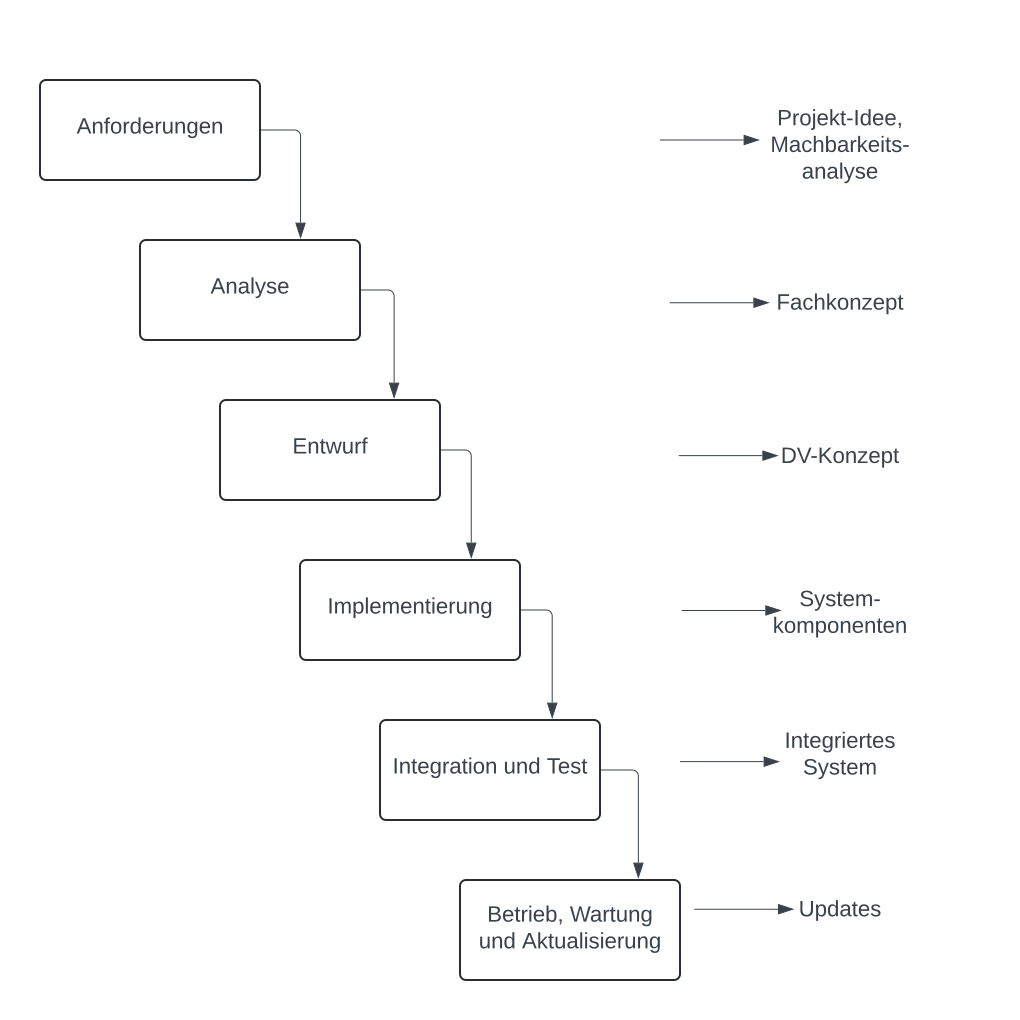
\includegraphics[scale=0.3]{part one/Uebersicht ueber die Phasen des Entwicklungszyklus/img/wasserfallmodell}
    \caption{Phasen des Wasserfallmodells. (Quelle: in Anlehnung an \cite[318, Abbildung 14-3]{AABG14n})}
    \label{fig:wasserfallmodell}
\end{figure}


\noindent
Vorgehensweisen, die auf dem Wasserfallmodell beruhen, sind das \textbf{V-Modell 97} und der \textbf{Team Software Process (TSP)} des Software Engineering Institute der Carnegie Mellon University.\\

\noindent
Das \textbf{Wasserfallmodell} ist ein \textit{sequentielles} und \textit{dokumentengetriebenes} Phasenmodell:

\blockquote[{\cite[319]{AABG14n}}]{
    Während aller Phasen der Systementwicklung, sowohl bei Individualentwicklung
    wie auch bei der Einführung von Standardsoftware, sollte beispielsweise durch
    Modelle auf Strategie- und Prozessebene, Machbarkeitsstudie, Fachkonzept, DVKonzept, Implementierungsdokumentation
    und Testbeschreibungen eine permanente Dokumentation erfolgen.
}

\subsection{Phasen des Wasserfallmodells}


\subsubsection{Anforderungen (1)}
In dieser Phase arbeitet man sich in die Fachlichkeit ein\footnote{
die sog. \textit{Domänenanalyse}, die vor der Erarbeitung der Anforderungen stattfindet. S.a. Abschnitt~\ref{sec:domanenanalyse}
}, um das Geschäftsfeld des Kunden zu verstehen und im folgenden eine ``gemeinsame Sprache`` zu sprechen, wenn es um die Anforderungen der Software geht.\\
Danach wird mit dem Kunden ein Konzept erstellt, das die Funktionalität der Software im ersten Release beschreibt und im sogenannten \textbf{Lastenheft}\footnote{
oder auch \textit{Vision \& Scope}. Hier finden sich auch Angaben zu der erhofften Wirtschaftlichkeit des geplanten Produkts.
} festgehalten wird.\\
Es werden auch \textbf{nicht-funktionale} Anforderungen festgehalten, wie bspw. Antwortzeiten, Datenmengen und erwartete Auslastung des Systems (bspw. Benutzerzahlen zu Stoßzeiten).\\
Die umzusetzende Funktionalität wird anhand von \textbf{Anwendungsfällen} beschrieben.\\

\noindent
In diesem Kontext spricht man deswegen auch von \textbf{Requirements Engineering}.


\subsubsection{Analyse (2)}
In dieser Phase geht es darum, Ergebnisse aus der ersten Phase systematisch zu analysieren, um Zusammenhänge und Anläufe besser zu verstehen sowie die Vollständigkeit der Anforderungen zu überprüfen, um danach alles detaillierter zu spezifizieren.\\
Im Zuge dessen wird ein \textbf{Fachkonzept} erstellt, in dem fachliche Zusammenhänge und Geschäftsabläufe in einem Modell \textbf{formalisiert} werden, dem sogenannten \textbf{Domänen-Modell}; die Formalisierung hierbei ist sehr wichtig, um Zweideutigkeiten und Mißverständnisse zu vermeiden\footnote{
    In diesem Modell sind nicht nur Geschäftsregeln und -logik dokumentiert, sondern bspw. auch Wertebereiche von Eingabefeldern.
}.\\
Als Beschreibungssprache wird i.d.R. \textbf{UML} verwendet.\\

\noindent
In diesen  Modellen kommen keinerlei technische Details vor, damit man nicht Gefahr läuft, bereits in dieser Phase technische Details zu diskutieren, und sich klar auf die Anforderungen konzentriert.\\

\noindent
Anhand des erstellten Models und der Anforderungen können auch Schnittstellen nach Außen definiert werden, wie bspw. das GUI als Mensch-Maschine-Schnittstelle, oder Schnittstellen zu anderen Systemen (bspw. Import-/Exportschnittstellen).\\

\noindent
Da die Phase der Analyse eng mit der Phase der Anforderungen verknüpft ist, werden diese beiden Phasen häufig abwechselnd bearbeitet.


\subsubsection{Entwurf (3)}
In dieser Phase wird das in der Anforderungs-Phase erstellte \textit{Fachkonzept} zu einem \textbf{DV-Konzept} fortgesetzt:

\blockquote[{\cite[319]{AABG14n}}]{
    Das Ergebnis dieser Phase wird oftmals als DV-Konzept bezeichnet und enthält eine systematische Beschreibung
    der Daten-, Funktions-, Organisations- und Steuerungssicht des zu entwickelnden Systems.
}

\noindent
Es wird ein Modell des Softwaresystems erstellt und die Architektur des Systems geplant.\\
Anhand dessen können Entwickler zu erstellenden Programmcode, Strukturen und Muster vorschlagen und durchspielen um den für das umzusetzende System besten Ansatz zu finden.\\
Es werden Schnittstellen einzelner Module spezifiziert.\\
Auch hier wird wieder \textbf{UML} und objektorientierte Verfahren eingesetzt.\\

\noindent
\textit{Alpar et al.} merken an, dass dieser Schritt häufig komplex ist, und weisen auf eine weitere Unterteilung hin\footnote{vgl.~\cite[319]{AABG14n}}, und zwar in

\begin{itemize}
    \item \textit{Grobentwurf} (Hard-, Softwarearchitektur)
    \item \textit{Feinentwurf} (Screenlayouts, Programmentwürfe, detaillierte logische Schemata)
    \item \textit{Testplanung}
\end{itemize}

\subsubsection{Implementierung (4)}
Das \textit{DV-Konzept} wird durch Datenstrukturen und Algorithmen in die Konstrukte der Hard- und Softwareumgebung implementiert (vgl.~\cite[319]{AABG14n}).\\
Hierbei werden die Systemkomponenten bereits getestet.\\
Bei den Implementierungen können Top-Down- oder Bottom-Up-Ansätze verfolgt werden\footnote{
    Top-Down: Funktionen übergeordneter Module werden schrittweise durch detailliertere Low-Level Module realisiert. Bottom-Up: Detaillierte Module werden inkrementell in übergeordnete Komponenten integriert.
}.\\
Das Ergebnis dieser Phase sind \textbf{Programmcode} und \textbf{Datenbankschemen}.

\subsubsection{Test (5)}
Die einzelnen Subsysteme werden in das Gesamtsystem integriert und getestet (\textit{Systemtests}, \textit{Integrationstests}).\\
Auch die Einhaltung nicht-funktionaler Anforderungen wird überprüft (bspw. durch \textbf{Lasttest}).\\
Das Ergebnis dieser Phase sind \textbf{Testfälle} und \textbf{Testprotokolle}.

\subsubsection{Einführung und Wartung (6)}
Das System wird an den Kunden ausgeliefert und geht in den Produktiv- bzw. \textbf{Wirkbetrieb} über, danach wird es durch Fehlerbehebungen und Aktualisierungen \textit{gewartet}.
